\documentclass[a4paper,12pt]{article}
%spellchecker
% !TeX spellcheck = de

\usepackage{amssymb} % needed for math
\usepackage{amsmath} % needed for math
\usepackage[utf8]{inputenc} % this is needed for german umlauts
\usepackage[ngerman]{babel} % this is needed for german umlauts
\usepackage[T1]{fontenc}    % this is needed for correct output of umlauts in pdf
\usepackage[margin=2.5cm]{geometry} %layout
\usepackage{booktabs}



% this is needed for forms and links within the text
\usepackage{hyperref}  

% Generate the glossary
\usepackage[nonumberlist]{glossaries}
\makeglossary

% The following is needed in order to make the code compatible
% with both latex/dvips and pdflatex.
\ifx\pdftexversion\undefined
\usepackage[dvips]{graphicx}
\else
\usepackage[pdftex]{graphicx}
\DeclareGraphicsRule{*}{mps}{*}{}
\fi

%%%%%%%%%%%%%%%%%%%%%%%%%%%%%%%%%%%%%%%%%%%%%%%%%%%%%%%%%%%%%%%%%%%%%%
% Variablen                                 						 %
%%%%%%%%%%%%%%%%%%%%%%%%%%%%%%%%%%%%%%%%%%%%%%%%%%%%%%%%%%%%%%%%%%%%%%
\newcommand{\authorName}{Lena Gregor, Dominik Horn}
\newcommand{\auftraggeber}{Lehrstuhl für Datenbanksysteme TUM}
\newcommand{\auftragnehmer}{\authorName}
\newcommand{\projektName}{Wahl und Informationssystem für bayrische Landtagswahlen}
\newcommand{\tags}{\authorName, Pflichtenheft, TUM, Universität Augsburg, LMU}
\newcommand{\subtitle}{Technische Universität München, Datenbanksysteme WS19/20}
\newcommand{\glossarName}{Glossar}

%%%%%%%%%%%%%%%%%%%%%%%%%%%%%%%%%%%%%%%%%%%%%%%%%%%%%%%%%%%%%%%%%%%%%%
% PDF Meta information                                 				       %
%%%%%%%%%%%%%%%%%%%%%%%%%%%%%%%%%%%%%%%%%%%%%%%%%%%%%%%%%%%%%%%%%%%%%%
\hypersetup{
  pdfauthor   = {\authorName},
  pdfkeywords = {\tags},
  pdftitle    = {\projektName~(Pflichtenheft)}
} 

%%%%%%%%%%%%%%%%%%%%%%%%%%%%%%%%%%%%%%%%%%%%%%%%%%%%%%%%%%%%%%%%%%%%%%
% Custom setup                                                       % 
%%%%%%%%%%%%%%%%%%%%%%%%%%%%%%%%%%%%%%%%%%%%%%%%%%%%%%%%%%%%%%%%%%%%%%
\usepackage{pdfpages}
\usepackage{xcolor,colortbl} 
\definecolor{Blue}{rgb}{0.1,0.2,0.7}
\definecolor{TUMBlue}{HTML}{0065BD}
\definecolor{TUMSecondaryBlue}{HTML}{005293}
\definecolor{TUMSecondaryBlue2}{HTML}{003359}
\definecolor{TUMAccentBlue}{HTML}{64A0C8}
\definecolor{TUMAccentLightBlue}{HTML}{98C6EA}
\definecolor{lightBlue}{RGB}{157,195,230}


\newcolumntype{a}{>{\columncolor{TUMBlue}}c}
\newcolumntype{b}{>{\columncolor{lightBlue}}c}

\renewcommand{\arraystretch}{1.5}
 
%%%%%%%%%%%%%%%%%%%%%%%%%%%%%%%%%%%%%%%%%%%%%%%%%%%%%%%%%%%%%%%%%%%%%%
% Create a shorter version for tables. DO NOT CHANGE               	 %
%%%%%%%%%%%%%%%%%%%%%%%%%%%%%%%%%%%%%%%%%%%%%%%%%%%%%%%%%%%%%%%%%%%%%%
\newcommand\addrow[2]{\textcolor{black}{#1} &#2\\ \hline}

\newcommand\addheading[2]{\rowcolor{TUMBlue}\textcolor{white}{#1} & \textcolor{white}{#2}\\ \hline}
\newcommand\tabularhead{\begin{tabular}{|b|p{13cm}|}
\hline
}

\newcommand\addmulrow[2]{ \begin{minipage}[t][][t]{2.5cm}#1\end{minipage}% 
   &\begin{minipage}[t][][t]{8cm}
    \begin{enumerate} #2   \end{enumerate}
    \end{minipage}\\ }

\newenvironment{usecase}{\tabularhead}
{\hline\end{tabular}}

%%%%%%%%%%%%%%%%%%%%%%%%%%%%%%%%%%%%%%%%%%%%%%%%%%%%%%%%%%%%%%%%%%%%%%
% THE DOCUMENT BEGINS             	                              	 %
%%%%%%%%%%%%%%%%%%%%%%%%%%%%%%%%%%%%%%%%%%%%%%%%%%%%%%%%%%%%%%%%%%%%%%
\begin{document}
 \pagenumbering{roman}
 \begin{titlepage}
\maketitle
\thispagestyle{empty} % no page number

\begin{verbatim}












\end{verbatim}


  \begin{tabular}[t]{ll}
	Projekt:       & \quad \projektName \\[1.2ex]
	Auftraggeber:  & \quad \auftraggeber\\[1.2ex]
	Auftragnehmer: & \quad \auftragnehmer\\[1.2ex]
  \end{tabular}

\begin{tabular}{|p{3 cm}|p{3 cm}|p{5 cm}|}
\hline
\textbf{Version} & \textbf{Datum} & \textbf{Autor(en)} \\
\hline
\hline
1.0 & 04.11.2019 & \authorName \\
\hline
\end{tabular}
\end{titlepage}
         % Deckblatt.tex laden und einfügen
 \setcounter{page}{2}

 \tableofcontents          % Inhaltsverzeichnis ausgeben
 \clearpage
 \pagenumbering{arabic}
 
\section{Zielbestimmung}
%%%%%%%%%%%%%%%%%%%%%%%%%%%%%%%%%%%%%%%%%%%%%%%%%%%%%%%%%%%%%%%%%%%%%%
% Warum wird das Projekt gemacht?           						 %
%%%%%%%%%%%%%%%%%%%%%%%%%%%%%%%%%%%%%%%%%%%%%%%%%%%%%%%%%%%%%%%%%%%%%%
Der Freistaat Bayern möchte in Kooperation mit dem Lehrstuhl für 
Datenbanksysteme an der Technischen Universität München eine digitales 
Wahlinformations- und Stimmabgabesystem für Landtagswahlen mithilfe von 
Studierenden des Elite Software Engineering Masterstudiengangs aufbauen.
%
Das System soll dabei nicht nur die Ergebnisse für die Landtagswahlen 
2013 und 2018 analysier- und vergleichbar machen, e.g., die Sitzverteilung 
im Landtag, statistische Auswertung von Ergebnissen, Berechnung gewonnener
Mandate, sondern auch als sicheres Backendsystem für die elektronische 
Stimmabgabe im Wahllokal dienen. 
%
Es müssen die gesetzlichen Regelungen, Normen und Datenschutzaspekte
berücksichtigt werden. Als Basis gelten die Regelungen zur
Landtagswahl 2018


\subsection{Musskriterien}
% Requirements
\begin{usecase}
	\addheading{Nummer}{Die Anwendung ermöglicht es...} 
      \addrow{M01}{...WählerInnen Einzelstimmen abzugeben nach vorangestellter Freigabe durch eine(n) WahlhelferIn.}
      \addrow{M02}{...Im Echtbetrieb, das mehrere Stimmen gleichzeitig abgegeben werden}
      \addrow{M03}{...selbst im katastrophenfall persistierte Wahldaten zu recovern}
	\addrow{M04}{...dem oder der WahlhelferIn Stimmen in aggregierter Form einzugeben.}
	\addrow{M05}{...Daten von vergangenen Wahlen mit Hilfe einer CSV-Datei fehlerfrei in das System einzuspeisen und statistisch auszuwerten.}
	\addrow{M06}{...bei der statistischen Auswertung die Verteilung der Sitze, die Auswertung für die Direkt- und Listenmandate und die Anzahl der Stimmen pro Partei einzusehen.}
	\addrow{M07}{...pro Stimmkreis die Einzelstimmen zu Stimmkreisergebnissen vorzuaggregieren.}
	\addrow{M08}{...erst nach Abschluss einer Wahl diese statistisch Auszuwerten, e.g., um Wahlbeeinflussung oder timed-attacks auf das Wahlgeheimniss zu verhindern.}
	\addrow{M09}{Die Anwendung speichert Erst- und Zweitstimmen getrennt voneinander um das Wahlgeheimnis und Datenschutzaspekte zu respektieren.}
      \addrow{M10}{Das System beachtet alle relveanten gesetzlichen Vorgaben für bayrische Landtagswahlen}
\end{usecase}

\subsection{Sollkriterien}
\begin{usecase}
	\addheading{Nummer}{Beschreibung} 
	\addrow{S01}{Die Anwendung ermöglicht es dem Anwender die Ergebnisse von unterschiedlichen Wahlen in einer Ansicht zu vergleichen.}
      \addrow{S02}{Die Oberfläche zur statistischen Auswertung ist frei zugänglich, die zur Stimmabgabe (durch Wähler oder Wahlhelfer/ -leiter) je nur für Berechtigte.}
      \addrow{S03}{Das System ist hinreichend gegen unbefugte Zugriffe abgesichert, sodass es akzeptabel wäre im Realbetrieb}
\end{usecase}
\subsection{Kannkriterien}
\begin{usecase}
	\addheading{Nummer}{Beschreibung} 
	\addrow{K01}{Die Anwendung kann bei der statistischen Auswertung die Ergebnisse auf der Landkarte visualisieren}
      \addrow{K02}{Stimmabgaben können als gültig und ungültig ausgewertet werden.}
	\addrow{K03}{WahlleiterInnen können bereits eingegebene Stimmen korrigieren, beispielsweise nach einer Neuauszählung}
\end{usecase}

\subsection{Abgrenzungskriterien}
\begin{usecase}
      \addheading{Nummer}{Das System...} 
      \addrow{A01}{...Dient nicht als E-Voting Plattform sondern ist lediglich imstande Stimmen von WählerInnen in Wahlkabinen entgegen zu nehmen}
	\addrow{A02}{...kann nicht die Berechtigung von WählerInnen überprüfen.}
	\addrow{A03}{...verarbeitet und berechnet keine juristischen Ausnahmefälle, die bei den Wahlen 2013 und 2018 nicht relevant waren.}
\end{usecase}

\section{Technische Umsetzung}
Dieser Abschnitt widmet sich der geplanten technischen Realisierung
des Systems. Zunächst werden dazu anhand der Einsatzszenarien die Implementierungsidee
grob vorgestellt. Im darauf folgenden Abschnitt findet sich eine tabelarische 
Auflistung aller eingesetzten Technologien. Abschließend
wird der jeweilige Implementierungsansatz für alle Musskriterien beschrieben.

\subsection{Produkteinsatz und Umgebung}
Die Anwendung ist konzipiert und entwickelt um die Stimmabgabe 
zu bayrischen Landtagswahlen (Erst-, Zweitstimme) durch wahlberechtigte
Personen, sowie die (statistische-) Auswertung von Wahlergebnissen zu ermöglichen. 
%
Das System wird in verschiedenen Gebieten eingesetzt:

\begin{center}
\begin{tabular}{|m{5cm}|m{10cm}|}
	\hline
  \rowcolor{TUMBlue} \textcolor{white}{\textbf{Einsatzgebiet}} & \textcolor{white}{\textbf{Prozesse}} \\
  \hline
  Wahllokal & Abgabe von Einzelstimmen durch WählerInnen und batch Stimmeintragung durch WahlhelferInnen \\
	\hline
  Bürgerlicher Gebrauch & (statistische-)Analyse von Wahlergebnissen \\
  \hline
  Staatlicher Gebrauch & (statistische-)Analyse von Wahlergebnissen, Import von alten Wahlergebnissen \\
	\hline
\end{tabular}
\end{center}

Die (statistische-) Analyse und Auswertung von Wahlergebnissen erfolgt in einer frei zugänglichen
Weboberfläche, welche auf ein Backendsystem zur Datenbeschaffung zugreift. 
Während eines Wahlvorgangs sind Daten zum aktuellen Vorgang nicht (statistisch-) Auswertbar,
unter anderem um eine Beeinflussung oder Verfälschung des Wahlausgangs zu vermeiden.
Ebenso stellt das System sicher, dass keine Rückschlüsse auf einzelne durch das Auswertungstool
möglich sind.
%
Das Interface zur Stimmabgabe sowie die von WahlhelferInnen und WahlleiterInnen zu benutzenden Oberflächen sind 
ebenfalls mit Webtechnologien implementiert, jedoch Zugriffbeschränkt und nicht übers Internet aufrufbar. Sie greifen
auf das selbe Backendsystem wie die (statistische-) Analyse Oberfläche zu.
%
Der durchgängige Einsatz von Webtechnologien senkt unter anderem den Projektaufwand, da Entwickler sich nur in 
einem einzigen Technologiestack für das gesamte System bewegen müssen. Weiterhin sind insbesondere 
Webtechnologien dafür geeignet Geräte- und bildschirmgrößen-unabhängige Software zu erstellen. Dies ist wichtig
da es unpraktikabel ist sich vorab bei Wahlautomaten und (statistischen-)Auswertungsgeräten festzulegen.
%
Die Implementierung des Backendsystems erfolgt als minimale Softwareschicht auf einem externen 
Rechner, fortan \textit{server} genannt. Jede Benutzeroberfläche schickt alle Anfragen, egal ob lesend oder schreibend, 
an den Server. Dieser führt die jeweilige Operation aus und liefert gegebenfalls hervorgebrachte
Anfrageergebnisse wieder zurück an den Rechner auf welchem die Benutzeroberfläche angezeigt wird, fortan \textit{client}.

Jede Personengruppe kann zu jeder Zeit immer nur auf die für sie relevanten Interfaces zugreifen.
Dies steigert primär die intuitivität der Benutzeroberfläche und minimiert potentielle Verwirrung
bei Benutzern. Die Absicherung des Systems beruht hingegen explizit nicht auf den getrennten 
Oberflächen. Vielmehr wird das Backendsystem durch Nutzerauthentifizierung der WahlleiterInnen und 
WahlhelferInnen, sowie Authentifizierung der einzelnen Wahllokale gesichert. Hierzu erhält jede(r)
WahlhelferIn und WahlleiterIn und jedes Wahllokal vor jeder Landtagswahl einen sich je unterscheidenden 
Zugriffscode auf einem staatlich gesicherten, externen Kommunikationskanal zugesandt. Dieser
ist jeweils nur für genau die vorgesehene Tätigkeit am vorgesehenen Ort verwendbar.

Zur Persistierung von Daten durch das Backendsystem wird ein zugriffsgesichertes Datenbanksystem eingesetzt. Dieses
wird exklusiv von der durch das Projektteam implementierten Softwareschicht auf dem server angesprochen.
Das heißt, dass die Backendsoftware lediglich als Proxy zwischen BenutzerIn und Datenbanksystem agiert. Sämtliche 
Datenzugriffe erfolgen stets authentifiziert, gefiltert und werden protokoliert. 
%
Der Einsatz eines DBMS wird durch mehrere inhärente Vorteile begünstigt:

\begin{itemize}
      \item Parallele OLAP Abfragen ohne Zusatzaufwand möglich, i.e., mehrere BenutzerInnen können 
            gleichzeitig ungehindert voneinander `die Wahlergebnisse statistisch auswerten.
      \item Mehrbenutzer OLTP out-of-the-box, i.e., mehrere WählerInnen und WahlhelferInnen können parallel Stimmen
            eintragen.
      \item Hohe Ausfallsicherheit, i.e., das System läuft stabil über längere Zeiträume
      \item Recovery Funktionalität, i.e., falls ein Unglück geschieht (Brand im Datencenter, Stromausfall) 
            oder der Server abstürzt gehen keine Daten verloren, solange die entsprechenden DBMS features 
            (logging, backup) genutzt werden
      \item Die Datenzugriffschnittstelle ist standartisiert und flexibel (SQL)
      \item Integritätsbedingungen werden über das Datenbankschema automatisch realisiert
\end{itemize}

\subsection{Eingesetzte Technologien}
Der vorherige Abschnitt identifiziert zur Umsetzung des Systems folgende Softwarekomponenten:
\begin{itemize}
      \item Datenbanksystem zur Persistierung von Anwendungsdaten, d.h., Wahldaten zur bayrischen Landtagswahl
      \item Server software zur Annahme und Bearbeitung von Clientanfragen, insbesondere auch zur Ansteuerung des Datenbanksystems
      \item Client software, je eines für die Stimmabgabe, für Wahlhelfer, Wahlleiter und zur (statistischen-) Auswertung von Wahlergebnissen 
\end{itemize}
Im folgenden werden die Haupttechnologien zur Umsetzung dieser Systemkomponenten tabelarisch aufgelistet. Abbildung \ref{fig:architecture} zeigt
deren Interaktion und Aufbau graphisch.

\begin{center}
      \begin{tabular}{|m{4cm}|m{2.5cm}|m{8.5cm}|}
            \hline
        \rowcolor{TUMBlue} \textcolor{white}{\textbf{Funktion/Gebiet}} & \textcolor{white}{\textbf{Eingesetzte Technologie}} & \textcolor{white}{\textbf{Erläuterung}} \\
        \hline
        Programmiersprache & TypeScript & TypeScript ist eine von Microsoft entwickelte Programmiersprache, welche JavaScript hauptsächlich um statische Typisierungsfähigkeiten ergänzt. Sie ist die Implementierungssprache für alle Softwarebereiche dieses Projekts \\
        \hline
        Datenbanksystem & PostgreSQL & PostgreSQL ist ein von der Industrie großflächig eingesetztes kostenfreies DBMS mit sehr guter Reputation und erprobtem Produktiveinsatz in großen Anwendungen \\
        \hline
        Server & NodeJS & NodeJS ermöglicht es Plattformunabhängig JavaScript code auszuführen. Hier dient es dazu die Serversoftware auszuführen \\
        \hline
        Serverschnittstelle & Apollo Server & Apollo Server implementiert die notwendige serverseitige Funktionalität um auf GraphQL Anfragen zu antworten. Jeder request wird auf einen resolver-Funktion gemapped, welche sich darum kümmert die angeforderte funktion (Daten lesen, Daten schreiben) auszuführen. \\
        \hline
        Ansprechen Serverschnittstelle & Apollo Client & Apollo Client implementiert die notwendige clientseitige Funktionalität um GraphQL Anfragen an einen Server zu schicken und die Antworten zu empfangen \\
        \hline
        Frontend UI & React & React ist ein von Facebook entwickeltes UI-Framework und wird zur Darstellung sämmtlicher Inhalte verwendet \\
        \hline
        Frontend UI & Ant Design & Ant Design ist eine React Component Library, welche viele nützliche GUI-Elemente vorgefertigt bereitstellt \\
        \hline
      \end{tabular}
\end{center}

\begin{figure}[h!]
      \centering
      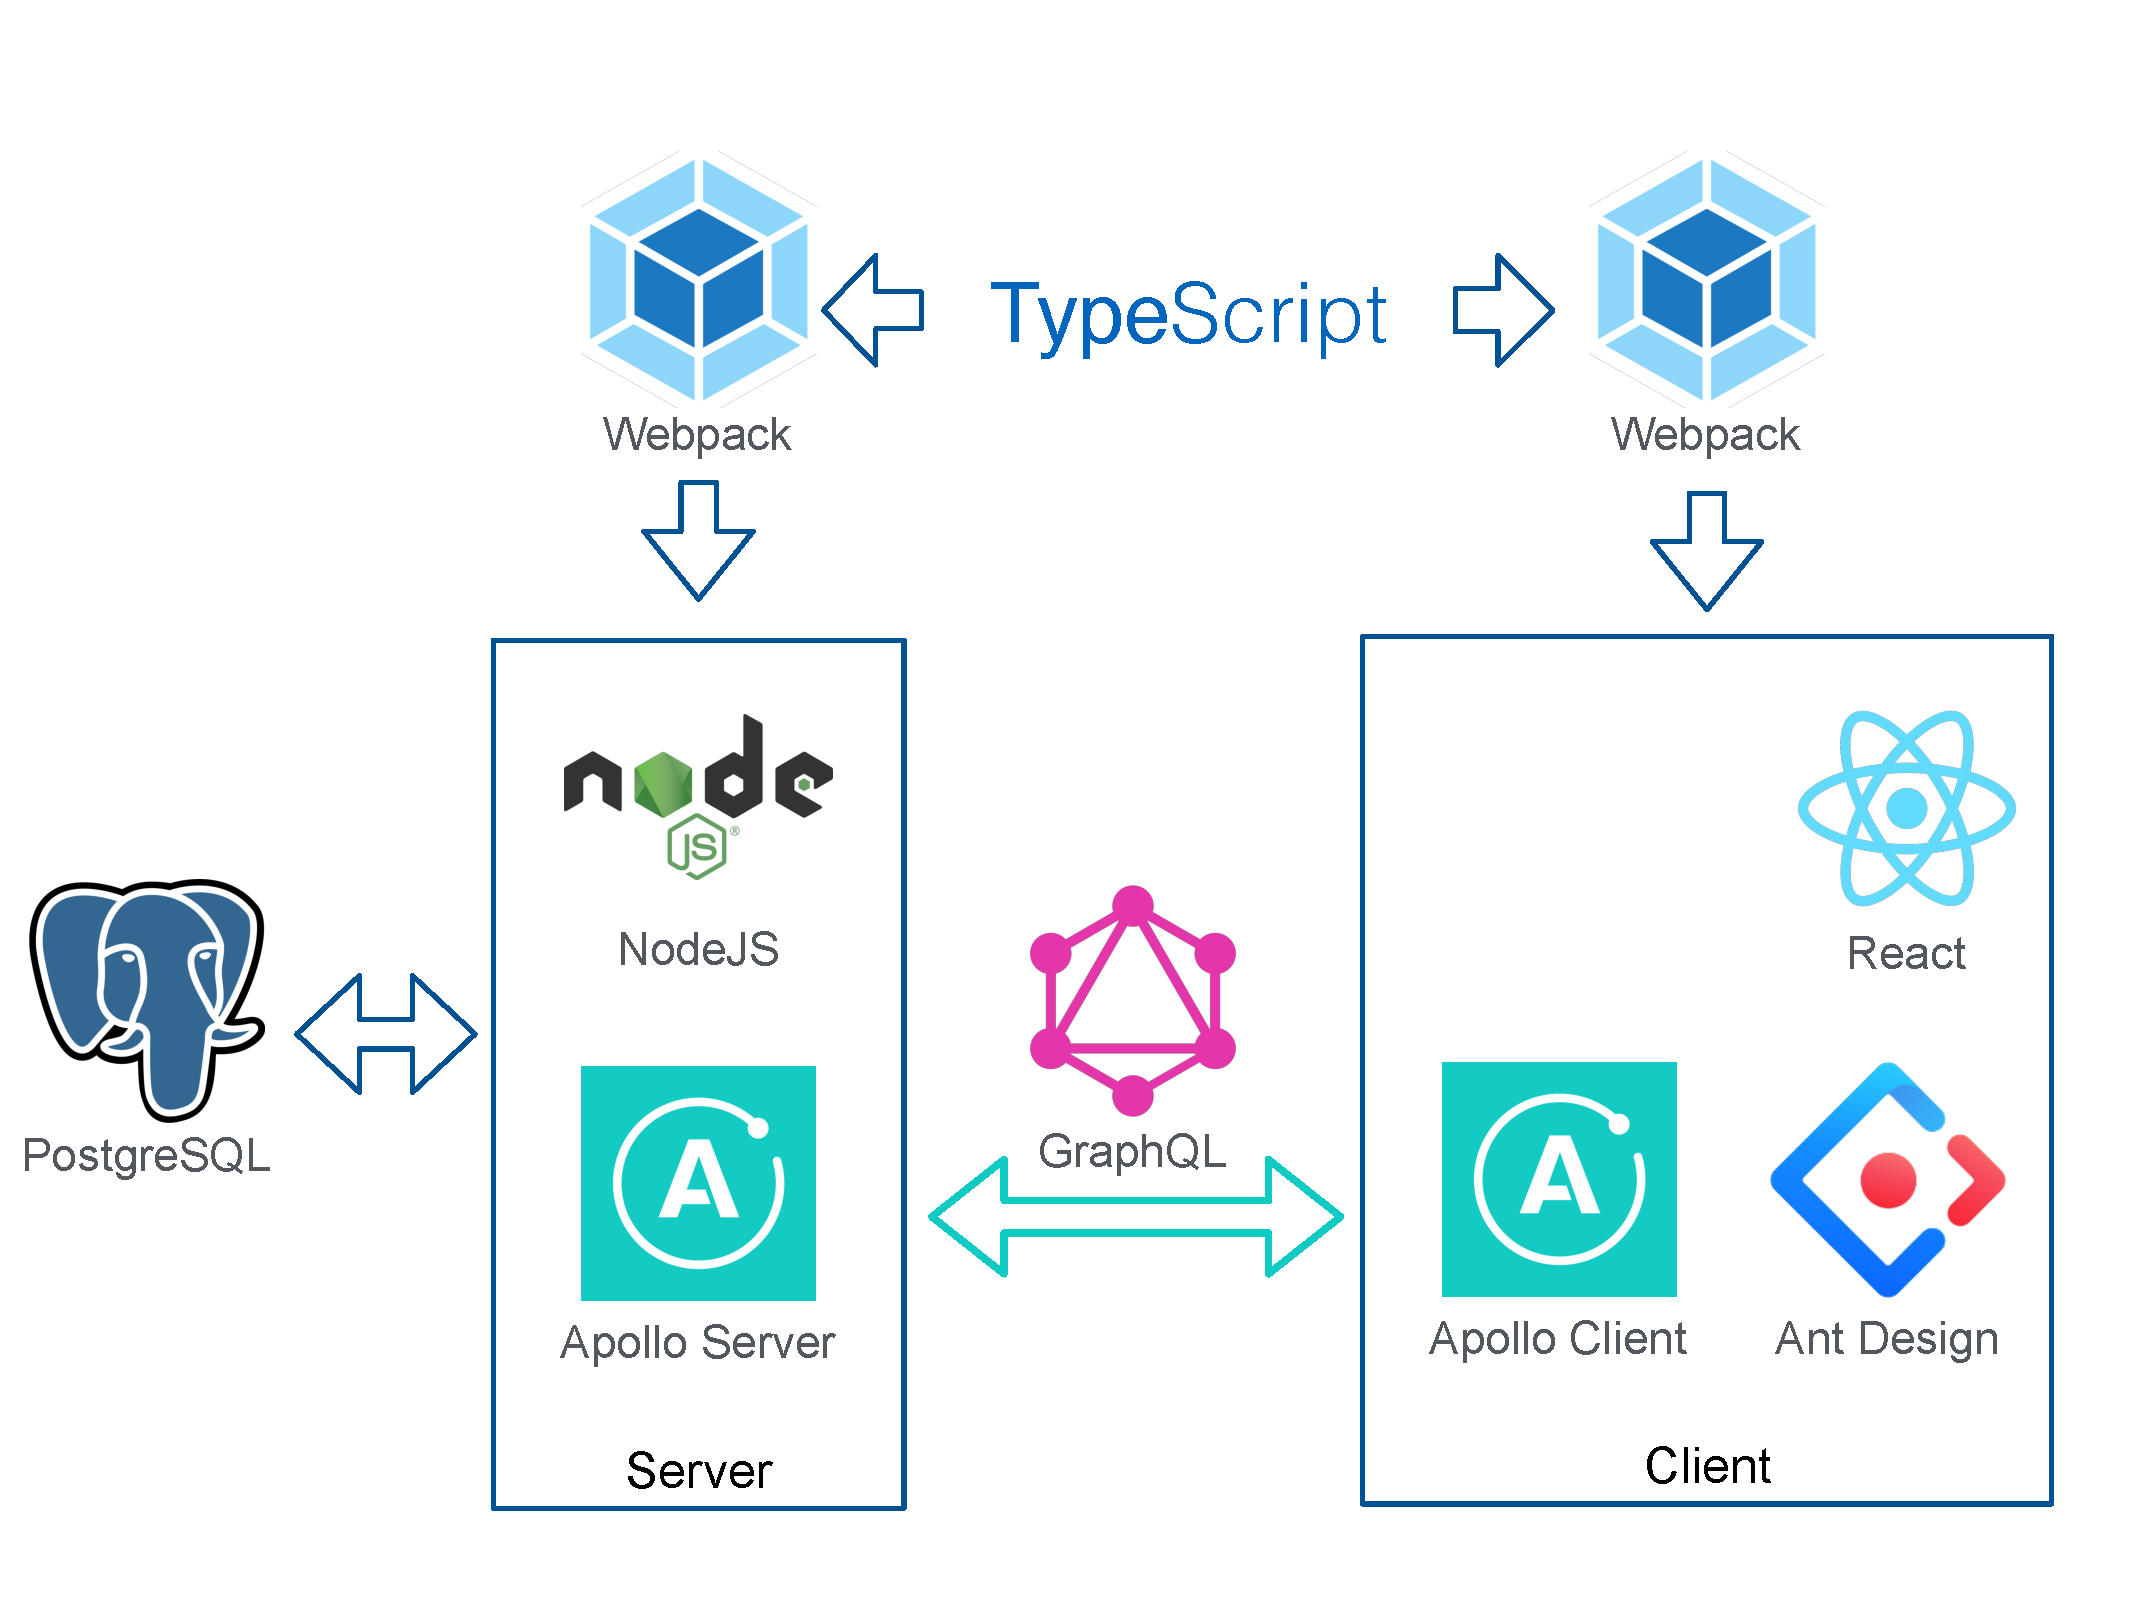
\includegraphics[width=\textwidth]{architecture.pdf}
      \caption{Illustrierung der Architektur und Interaktion von Systemkomponenten}
      \label{fig:architecture}
\end{figure}

\clearpage

\subsection{Erreichen der Zielsetzung}
Die definierten Kriterien und Systemeigenschafften werden durch die eingesetzten Technologien 
offensichtlich erreicht, sofern dieser Abschnitt sie nicht gesondert nennt.

\begin{usecase}
	\addheading{Nummer}{Zielsetzung wird erreicht, weil:} 
      \addrow{M01}{Der oder die WahlhelferIn in einer separaten Oberfläche die individuelle Freigabe für jede Instanz der Stimmabgabeoberfläche im Wahllokal erteilt. Danach kann der oder die WählerIn genau eine Erst- und Zweitstimme- über die Stimmabgabeoberfläche in der Wahlkabine abgeben.}
      \addrow{M02}{Das eingesetzte DBS PostgreSQL ist performant genug um ein Mehrbenutzer-OLTP Szenario plausibel zu ermöglichen.}
      \addrow{M03}{Das eingesetzte DBS verfügt über ausreichen Backup und Recovery Funktionalität.}
	\addrow{M07}{Dies wird über materialized Views im DBS erreicht.}
	\addrow{M08}{Der lesende Datenzugriff kann für die Wahldauer untersagt werden, beispielsweise auf DBS-Level.}
      \addrow{M10}{Datenschutz, Wahlgeheimnis u.ä. sind durch das Datenmodel und die Absicherung des Systems gewährleistet. Die restlichen Vorgaben werden von der Implementierung und dem Datenmodel umgesetzt.}
      \addrow{S02}{Getrennte Oberflächen welche sich ggf. hinter einer für Webanwendungen üblichen Zugriffskontrolle befinden.}
      \addrow{S03}{Sichere Webanwendungen können diese Garantien genauso sehr treffen wie andere vergleichbare Implementierungsansätze, wie an Ihrem breiten Produktiveinsatz durch viele Spitzenunternehmen ersichtlich ist.}
\end{usecase}

\section{GUI Mockups}
% TODO

\section{Datenmodell}
Die grundlegenden zu verwaltenden Produktdaten ergeben sich aus der folgenden Liste von
identifizierten Entitäten:
\begin{itemize}
  \item \textbf{Wahl} - Repräsentation einer einzelnen Wahl an einem festen Datum. 
        Durch letzteres Merkmal ist es möglich mehrere Wahlen in einem Jahr festzuhalten.
  \item \textbf{Stimme} - Jede(r) WählerIn besitzt je eine Erst- und Zweitstimme, welche er oder sie in Ihrem
        Stimmbezirk für KandidatInnen abgeben können. Mit der Erststimme wählt eine wahlberechtigte Person
        primär den oder die von ihr bevorzugten DirektkandidatIn ihres Stimmkreises. Über die Zweitstimme wählt 
        jede wahlberechtigte Person genau einen Kandidaten einer Liste aus ihrem Regierungsbezirk. Das prozentuale
        Gesamtabschneiden einer Partei aus kombinierten Erst- und Zweitstimmen ist jedoch ebenso für das 
        Wahlergebnis relevant.
  \item \textbf{Regierungsbezirk} - Bayern ist in sieben Regierungsbezirke unterteilt: Oberbayern,
        Niederbayern, Schwaben, Ober-, Unter-, Mittelfranken und Oberpfalz. Jeder Regierungsbezirk
        hat eine unterschiedliche Anzahl zu vergebender Direkt- und Listenmandate
  \item \textbf{Stimmkreis} - Regierungsbezirke sind gemäß Bevölkerungszahlen in Stimmkreise aufgeteilt.
        Jeder Stimmkreis ist widerum in ein oder mehrere Stimmbezirke unterteilt. Pro Stimmkreis wird ein(e)
        DirektkandidatIn gewählt
  \item \textbf{Stimmbezirk} - Die Stimmabgabe erfolgt in Stimmbezirken
  \item \textbf{KandidatIn} - Eine sich zur Wahl stellende Person mit notwendigen persönlichen Angaben. 
        Insbesondere kann ein(e) KandidatIn als DirektkandidatIn für einen Stimmkreis aufgestellt sein.
  \item \textbf{Mandat} - Mandate für den Bayrischen Landtag können von KandidatInnen im Rahmen einer Landtagswahl
        errungen werden. Hierbei wird zwischen Direktmandaten, Listenmandaten und Ausgleichsmandaten unterschieden.
  \item \textbf{Partei} - KandidatInnen können Mitglied einer Partei sein und sich von dieser für einen Listenplatz
        aufstellen lassen
  \item \textbf{Liste} - Jede Partei kann pro Regierungsbezirk eine Liste mit KandidatInnen, welche Mitglieder der 
        Partei sind, aufstellen.
\end{itemize}

\begin{center}
	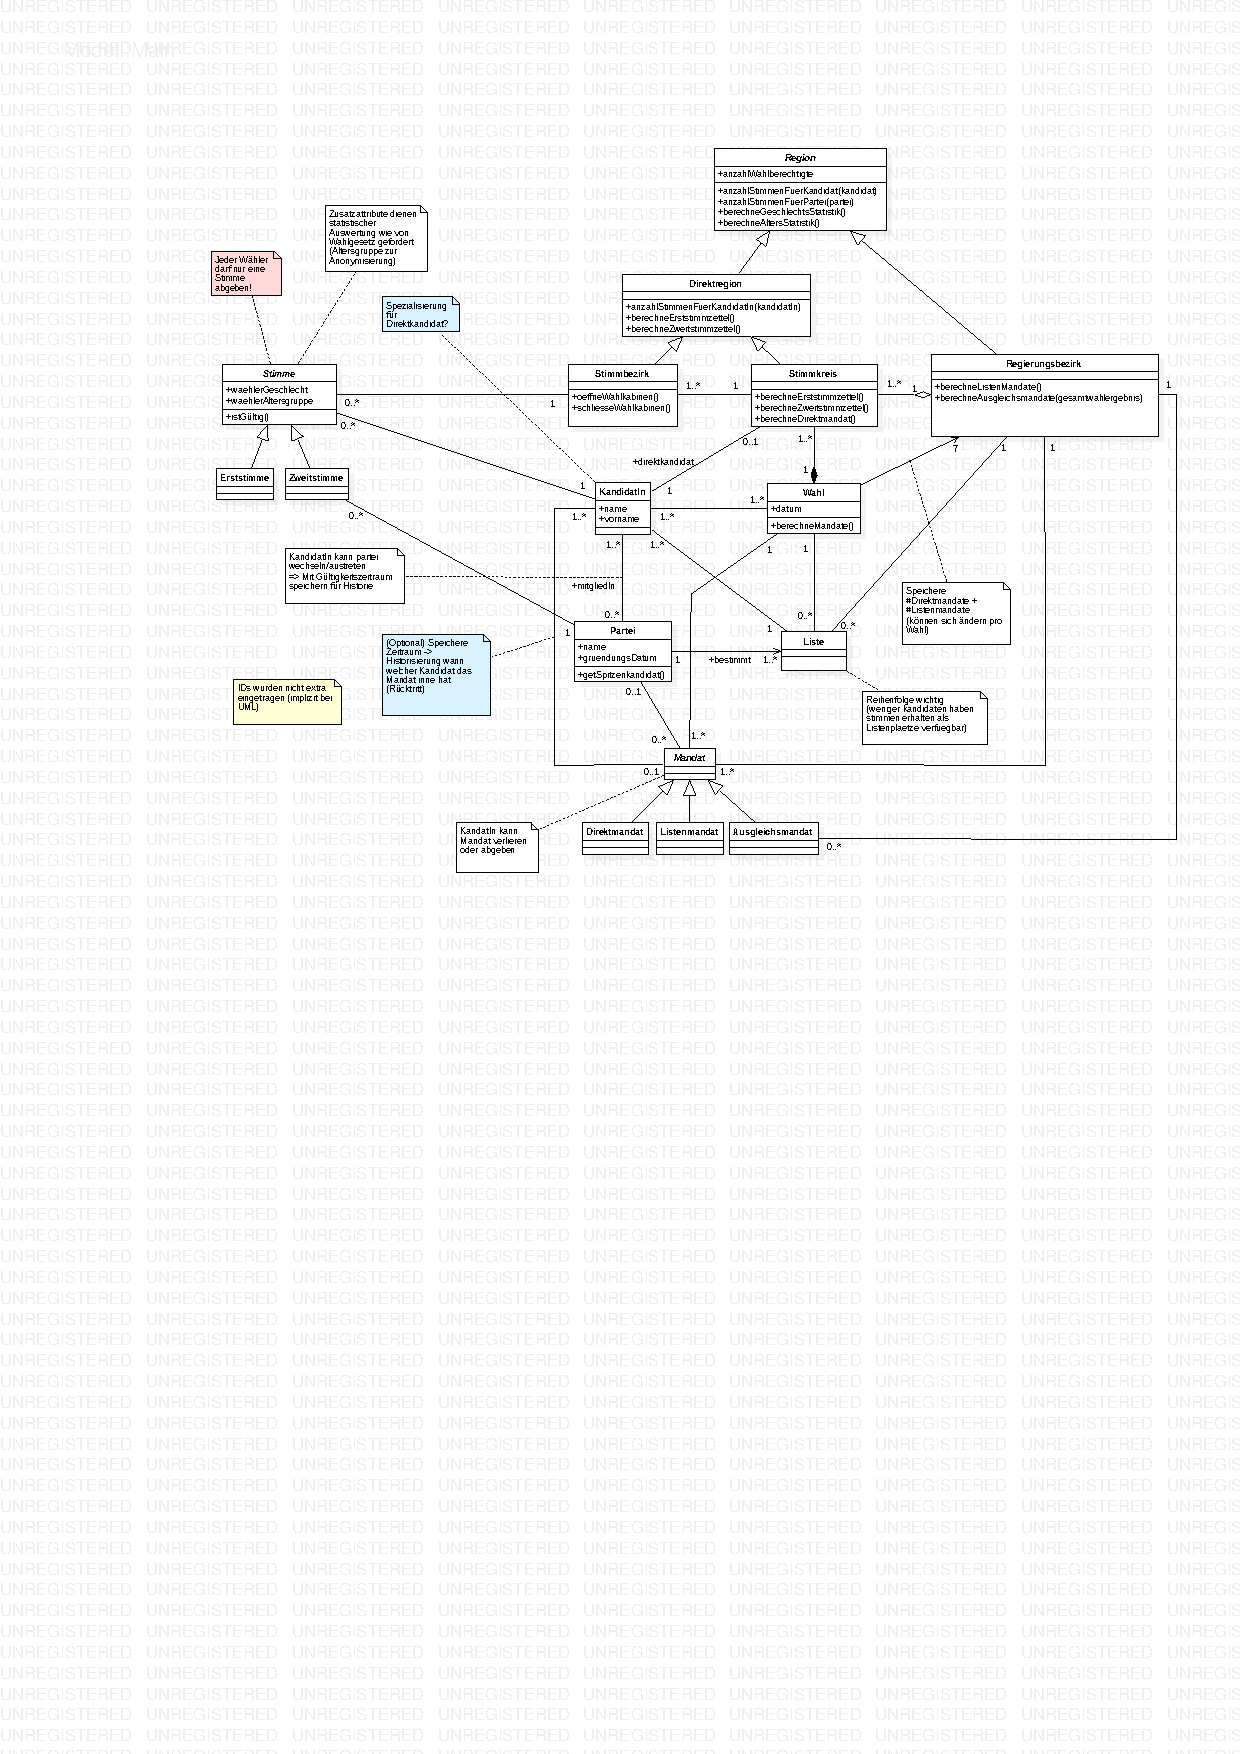
\includegraphics[width=\textwidth]{../model.pdf}
\end{center}

\section{Globale Testfälle und Szenarien}
\begin{center}
      \begin{tabular}{|m{3.5cm}|m{12cm}|}
        \hline
        \rowcolor{TUMBlue} \textcolor{white}{\textbf{Szenario}} & \textcolor{white}{\textbf{Abnahmekriterium}} \\
        \hline
        Stimmabgabe & 10~ Stimmabgaben können pro Sekunde erfolgen \\
        \hline
        (statistische-) Auswertung & Zur voraussichtlichen Hauptlastzeit unmittelbar nach Datenfreigabe zum Abschluss des Wahlvorgangs 
            bleibt das System performant. Es muss hierzu möglich sein 100 Analyseanfragen pro Sekunde zu bearbeiten \\
        \hline
      \end{tabular}
\end{center}

\clearpage
%%%%%%%%%%%%%%%%%%%%%%%%%%%%%%%%%%%%%%%%%%%%%%%%%%%%%%%%%%%%%%%%%%%%%%
% Begriffslexikon zur Beschreibung des Produkts						 %
%%%%%%%%%%%%%%%%%%%%%%%%%%%%%%%%%%%%%%%%%%%%%%%%%%%%%%%%%%%%%%%%%%%%%%
%\newglossaryentry{sortierschluessel}
%{
%  name=Sortierschlüssel,
%  description={ein Schlüssel, anhand dessen diese Einträge sortiert werden}
%}
\newglossaryentry{Technologiestack}
{
  name=Technologiestack,
  description={Sammlung aller verwendeten Technologien im Projekt. Gegebenenfalls hierarchisch sortiert wenn aufeinander aufbauend}
}
\newglossaryentry{Client}
{
  name=Client,
  description={Programm, dass die Dienste eines Servers in Anspruch nimmt}
}
\newglossaryentry{Server}
{
  name=Server,
  description={Rechner, der für andere in einem Netzwerk mit ihm verbundene Systeme bestimmte Aufgaben übernimmt und von dem diese ganz oder teilweise abhängig sind}
}
\newglossaryentry{Datenbanksystem}
{
  name=Datenbanksystem,
  description={Ein Datenbanksystem (DBS) ist eine systematisch strukturierte, langfristig verfügbare Sammlung von Daten einschließlich der zur Verwaltung notwendigen Software}
}
\newglossaryentry{OLAP}
{
  name=OLAP,
  description={Online Analytical Processing}
}
\newglossaryentry{OLTP}
{
  name=OLTP,
  description={Online Transaction Processing}
}


% Setze den richtigen Namen für das Glossar
\renewcommand*{\glossaryname}{\section{\glossarName}}

% Drucke das gesamte Glossar
\glsaddall
\printglossaries

% Trage das Glossar in das Inhaltsverzeichnis ein
\stepcounter{section}
\addcontentsline{toc}{section}{\numberline {\thesection} \glossarName}
\end{document}
